\documentclass[12pt]{article}
\usepackage{{../preamble}}
\graphicspath{{pics}}

\begin{document}
\chead{Problem Set 2}

%%%%%%%%%%%%%%%%%%%%%%%%%%%%%%%%%%%%%%%%%%%%%%%
%                  Definitions                %
%%%%%%%%%%%%%%%%%%%%%%%%%%%%%%%%%%%%%%%%%%%%%%%
\def\xdot{\dot X} \def\ydot{\dot Y} \def\zdot{\dot Z}
\def\kdot{\dot k} \def\ccdot{\dot c} \def\ddt{\frac{d}{dt}}
\def\dfdk{\frac{\partial F}{\partial K}}
\def\dfdl{\frac{\partial F}{\partial L}}
\def\plim{\lim\limits_{\phi\to 0}}
\def\ddp{\dfrac{\partial}{\partial \phi}}
\def\dgdp{\dfrac{\partial\gamma}{\partial \phi}}
\def\invphi{\sfrac{1}{\phi}}




%%%%%%%%%%%%%%%%%%%%%%%%%%%%%%%%%%%%%%%%%%%%%%%
%                Problem 1                    %
%%%%%%%%%%%%%%%%%%%%%%%%%%%%%%%%%%%%%%%%%%%%%%%
\section*{Problem 1}
\problem{Growth, saving, and $r-g$: Romer 2.6}{
    Piketty (2014) argues that a fall in the growth rate
of the economy is likely to lead to an increase in the difference between the real
interest rate and the growth rate. This problem asks you to investigate this issue
in the context of the Ramsey Cass Koopmans model. Specifically, consider a
Ramsey Cass Koopmans economy that is on its balanced growth path, and suppose
there is a permanent fall in $g$.

    \begin{enumerate}[label=(\alph*)]
    \item How, if at all, does this affect the $\kdot = 0$ curve?
    \end{enumerate} 
}


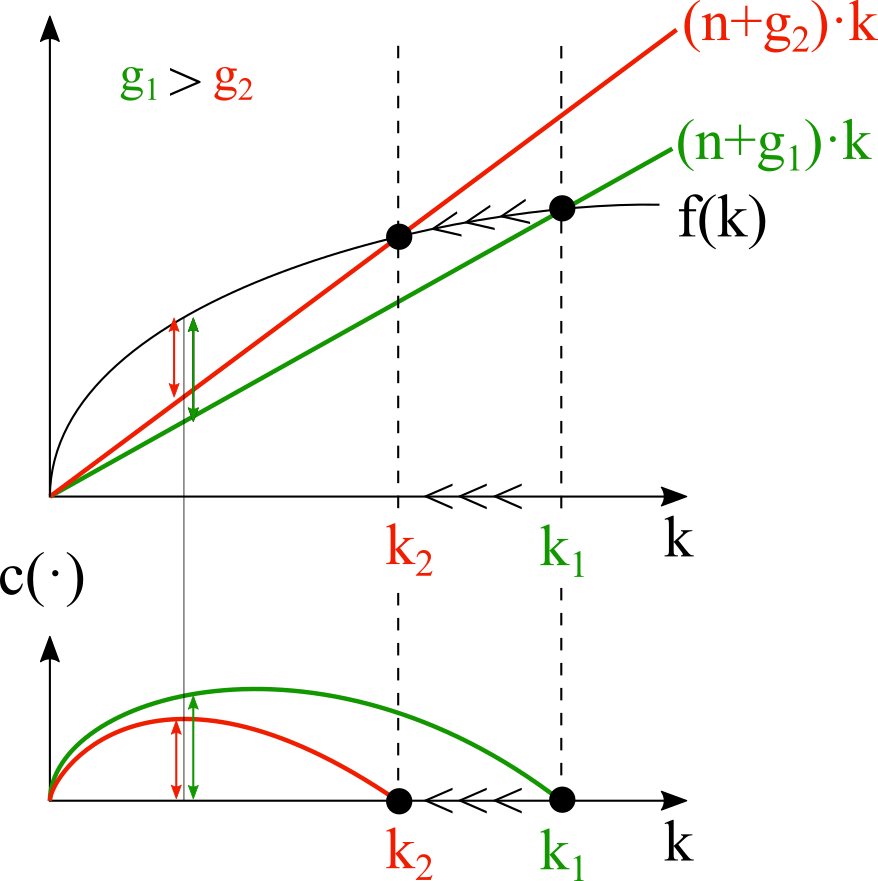
\includegraphics[width=0.5\textwidth]{1.a}


In the plot above, we can see a decrease in $g$
\begin{itemize}
    \item[$\implies$] a decrease in the slope of $(n+g)k$
    \item[$\implies$] increase in the $k$ where $f(k)-(n+g)k=0$
    \item[$\implies$] increase in the $k$ where the $\kdot=0$ curve meets the $k$ axis
\end{itemize}

A decrease in the slope of $(n+g)k$ also implies that the distance between $(n+g)k$ and $f(k)$ will be larger $\forall k$ between 0 and where $f(k)-(n+g)k=0$.

\noindent
So, overall, a decrease in $g$ implies a vertical and horizontal stretch outward for the $\kdot = 0$ curve.


%%%%%%%%%%%%%%%%%
%     Part b    %
%%%%%%%%%%%%%%%%%
\newpage\problem{}{
    \begin{enumerate}[label=(\alph*)]
    \setcounter{enumi}{1}
    \item How, if at all, does this affect the $\ccdot = 0$ curve?
    \end{enumerate} 
}

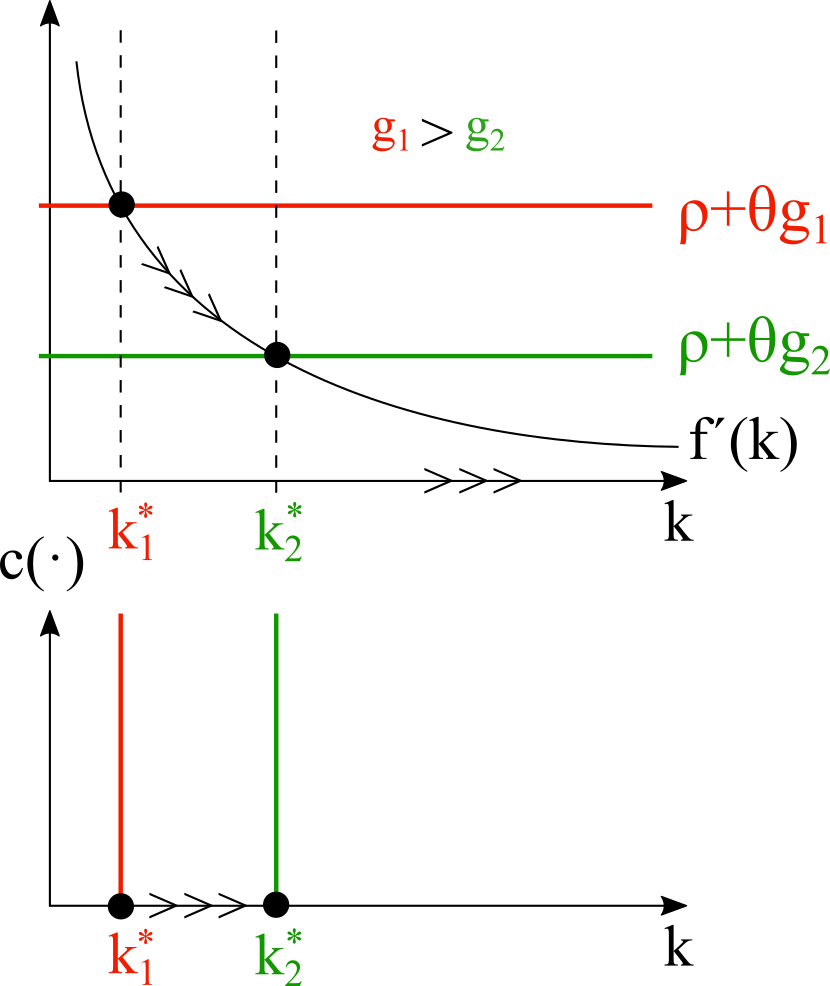
\includegraphics[width=0.5\textwidth]{1.b}

Because $f'>0$ and $f''<0$ by assumption, the plot of $f'$ is shaped as in the above plot. Then when $g$ has decreased from $g_1$ to $g_2$, the intersection with $f'$ occurs at a higher $k^*$. Since $\ccdot=0$ occurs when $f'=\rho+\theta g$ and $\rho, \theta$ are constants, then the $\ccdot=0$ curve shifts to the right to a higher $k^*$.
  

%%%%%%%%%%%%%%%%%
%     Part c    %
%%%%%%%%%%%%%%%%%
\newpage\problem{}{
    \begin{enumerate}[label=(\alph*)]
    \setcounter{enumi}{2}
    \item At the time of the change, does $c$ rise, fall, or stay the same, or is it not possible to tell?
    \end{enumerate} 
}

Since $k_1^* < k_2^*$ from the plot in part (b)
\begin{itemize}
    \item[$\implies$] immediately after the decrease from $g_1$ to $g_2$, $f'(k_1^*)>\rho+\theta g_2$.
    \item[$\implies$] $\dfrac{\ccdot}{c}\bigg|_{k=k_1^*,g=g_2} = \dfrac{f'(k_1^*) - \rho - \theta g_2}{\theta} > 0$
    \item[$\implies$] $\ccdot|_{k=k_1^*,g=g_2} > 0$
    \item[$\implies$] $c$ rises immediately after the decrease in $g$
\end{itemize}


%%%%%%%%%%%%%%%%%
%     Part d    %
%%%%%%%%%%%%%%%%%
\newpage\problem{}{
    \begin{enumerate}[label=(\alph*)]
    \setcounter{enumi}{3}
    \item At the time of the change, does $r-g$ rise, fall, or stay the same, or is it not possible to tell?
    \end{enumerate} 
}

Since there is no depreciation, the real interest rate $r$ is equal to the marginal product of capital $f'(k)$ (since the price of output is assumed to be 1).

\begin{align*}
    \intertext{So}
    r-g &= f'(k) - g
    \intertext{And immediately after the change in g,}
    f'(k_1^*) - g_1
    \intertext{changes to}
    f'(k_1^*) - g_2
    \intertext{Since $f'(k)$ remains unchanged at the time of the change but $g$ decreases from $g_1$ to $g_2$,}
    f'(k_1^*) - g_2 &>  f'(k_1^*) - g_1\\
    r|_{g_1}-g_2 &> r|_{g_1}-g_1
    \intertext{So, at the time of the change, $r-g$ increases.}
\end{align*}



%%%%%%%%%%%%%%%%%
%     Part e    %
%%%%%%%%%%%%%%%%%
\newpage\problem{}{
    \begin{enumerate}[label=(\alph*)]
    \setcounter{enumi}{4}
    \item In the long run, does $r-g$ rise, fall, or stay the same, or is it not possible to tell?
    \end{enumerate} 
}

\begin{align*}
    \intertext{Continuing my notation from parts (b)-(d), in the long run,}
    \lim_{t\to\infty}f'(k) &= f'(k_2^*)
    \intertext{So the change in $r-g$ in the long run will be}
    (r|_{g_2}-g_2) - (r|_{g_1}-g_1) &= (f'(k_2^*)-g_2) - (f'(k_1^*)-g_1) \\
        &= (\rho +\theta g_2 -g_2) - (\rho +\theta g_1-g_1) \\
        &= (\rho +(\theta-1) g_2) - (\rho +(\theta-1)g_1) \\
        &= (\theta-1) (g_2-g_1) \\
        &\begin{cases}
            >0 &\text{ if } \theta\in (0,1) \\
            <0 &\text{ if } \theta > 1
        \end{cases}
\end{align*}

Since there is no upper constraint on $\theta$ from the utility function ($\theta\in (0,1)$ and $\theta > 1$ both produce an upward sloping, convex function), then there is no way to tell, in general, if $r-g$ rises or falls without an estimate of $\theta$.


%%%%%%%%%%%%%%%%%
%     Part f    %
%%%%%%%%%%%%%%%%%
\newpage\problem{}{
    \begin{enumerate}[label=(\alph*)]
    \setcounter{enumi}{5}
    \item Find an expression for the impact of a marginal change in $g$ on the fraction of output that is saved on the balanced growth path. Can one tell whether this expression is positive or negative?
    \end{enumerate} 
}
\def\c{c^*} \def\y{y^*} \def\k{k^*} \def\s{s^*} \def\f{f(\k)} \renewcommand{\t}{\tau}
\begin{align*}
    \intertext{Denote optimal savings rate as $s^* = (y^* - c^*)/y^*$. First we can use the $\kdot=0$ condition of the balanced growth path, which implies:}
    \c &= \y - (n+g)\k
    \intertext{Then the savings rate on the balanced growth path is}
    \s &= \frac{\y-\c}{\y} \\[1em]
        &= \frac{(n+g)\k}{\y} \\[1em]
        &= \frac{(n+g)\k}{\f}
    \intertext{Differentiating with respect to $g$, we have}
    \frac{d\s}{dg}
        &= \frac{\k}{\f} + (n+g)\l[\frac{1}{\f}\frac{d\k}{dg} - \frac{\k}{\f^2}\frac{df(\k)}{dg} \r] \\[1em]
        &= \frac{\k}{\f} + (n+g)\l[\frac{1}{\f}\frac{d\k}{dg} - \frac{\k}{\f^2}f'(\k)\frac{d\k}{dg} \r] \\[1em]
        &= \frac{\k}{\f} + \frac{n+g}{\f^2}\l[\f - \k f'(\k)\r]\frac{d\k}{dg} \\[1em]
    \intertext{Since $\dfrac{n+g}{\f^2}>0$, we just need to determine the sign of the term in square brackets and $\dfrac{d\k}{dg}$. Starting with the term in the brackets: from our assumptions about the production function, we can determine that}
    f'>0, f''<0 &\implies f(k) > k f'(k) \\
        &\implies f(k) - k f'(k) > 0 \quad \forall k>0
    \intertext{We can think about this graphically: since the slope of $f$ is positive and always decreasing, the tangent to $f$ at any point is going to intersect the vertical axis above the origin (i.e., $>0$). $f(k) - k f'(k)$ is precisely the height above the origin where this tangent intersects the vertical axis. The figure below demonstrates this for a particular point $k$, but it holds generally anywhere in the domain of $f$.}
\end{align*}

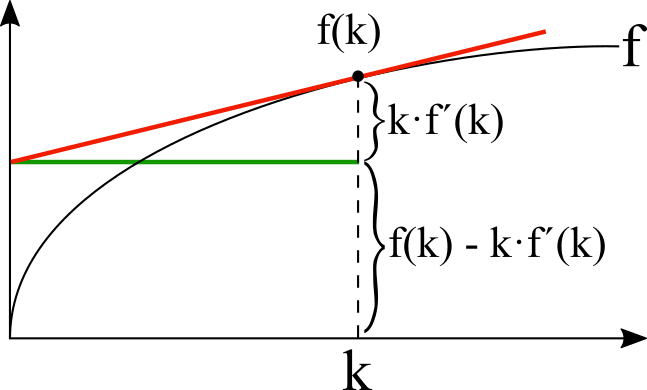
\includegraphics[width=0.5\textwidth]{1.f}

\begin{align*}
    \intertext{For the last term, we can totally differentiate the $\ccdot=0$ condition:}
    f'(\k) &= \rho + \theta g\\[0.5em]
    \implies  d[f'(\k)] &= d[\rho + \theta g]\\[0.5em]
    f''(\k) d\k &= \theta dg\\[0.5em]
    \frac{d\k}{dg} &= \frac{\theta}{f''(\k)} <0 \\[1em]
    \intertext{Since $f''<0$ by assumption.}
    \intertext{Which means that}
    \frac{d\s}{d\t} &=\underbrace{\frac{\k}{\f}}_{>0} + 
    \underbrace{ \frac{n+g}{\f^2} }_{>0}
            \underbrace{ \l[\f - \k f'(\k)\r] }_{>0}
            \underbrace{ \frac{d\k}{d\t} }_{<0} \\[1em]
        &<0
    \intertext{So the endogenous savings rate on the balanced growth path decrease as the investment income tax increases.}
\end{align*}

%%%%%%%%%%%%%%%%%
%     Part g    %
%%%%%%%%%%%%%%%%%
\newpage\problem{}{
    \begin{enumerate}[label=(\alph*)]
    \setcounter{enumi}{6}
    \item For the case where the production function is Cobb-Douglas, $f'(k^*) = k^\alpha$, rewrite your answer to part (f) in terms of $\rho, n, g, \theta,$ and $\alpha$. (Hint: Use the fact that $f'(k^*) = \rho + \theta g$.)
    \end{enumerate} 
}



%%%%%%%%%%%%%%%%%%%%%%%%%%%%%%%%%%%%%%%%%%%%%%%
%                Problem 2                    %
%%%%%%%%%%%%%%%%%%%%%%%%%%%%%%%%%%%%%%%%%%%%%%%
\newpage
\section*{Problem 2}
\problem{Capital taxation in the Ramsey-Cass-Koopmans model: Romer 2.10}{
    Consider a Ramsey-Cass-Koopmans economy that is on its balanced growth path. Suppose
that at some time, which we will call time 0, the government switches to a policy
of taxing investment income at rate $\tau$. Thus the real interest rate that households
face is now given by \[r(t) = (1-\tau) f'(k(t)).\] Assume that the government returns
the revenue it collects from this tax through lump-sum transfers. Finally, assume
that this change in tax policy is unanticipated.

    \begin{enumerate}[label=(\alph*)]
    \item How, if at all, does the tax affect the $\ccdot = 0$ locus? The $\kdot = 0$ locus?
    \end{enumerate} 
}
\def\kone{k^*_1} \def\ktwo{k^*_2}
\begin{align*}
    \intertext{To examine the effects on the $\ccdot=0$ locus, we set $\ccdot=0$ in the consumption Euler equation. This give}
    r(t) &= \rho + \theta g
    \intertext{Before the policy is introduced, we know $f'(k)=r(t)$ because firms are operating under a CRS production function in a competitive market. So let $\kone$ denote $k$ when $\ccdot=0$ before the tax is introduced, thus}
    f'(\kone) &= \rho + \theta g
    \intertext{After the tax is introduced, $r(t)=(1-\tau) f'(k(t))$, so let $\ktwo$ denote $k$ when $\ccdot=0$ after the tax is introduced, satisfying}
    (1-\tau)f'(\ktwo) &= \rho + \theta g\\[1em]
    f'(\ktwo) &= \frac{\rho + \theta g}{1-\tau}
    \intertext{Since $\tau\in(0,1)$, then $(1-\tau)^{-1}\in(1,\infty)$,so }
    \frac{\rho + \theta g}{1-\tau} &> \rho + \theta g \\[1em]
    f'(\ktwo) &> f'(\kone)
    \intertext{Because $f'>0$ and $f''<0$, this implies}
    \ktwo &< \kone
    \intertext{So, the $\ccdot=0$ locus is shifting left from a vertical line (in $k-c$ space) at $\kone$ to a vertical line at $\ktwo$.}
\end{align*} 

\newpage
\begin{align*}
    \intertext{To examine the effects on the $\kdot=0$ locus, we set $\kdot=0$ in the intensive form of the equation of motion for capital. This gives}
    c &= f(k) - (n+g)k
    \intertext{This equation is not related to $r(t)$ and does no change the $\kdot=0$ path through $k-c$ space. The new tax only changes how households trade off consumption for saving and where the $\ccdot=0$ locus intersects the $\kdot=0$ path.}
\end{align*} 

%%%%%%%%%%%%%%%%%
%     Part b    %
%%%%%%%%%%%%%%%%%
\newpage\problem{}{
    \begin{enumerate}[label=(\alph*)]
    \setcounter{enumi}{1}
    \item How does the economy respond to the adoption of the tax at time 0? What are the dynamics after time 0?
    \end{enumerate} 
}
{
\begin{wrapfigure}{l}{0.5\textwidth}
  \begin{center}
    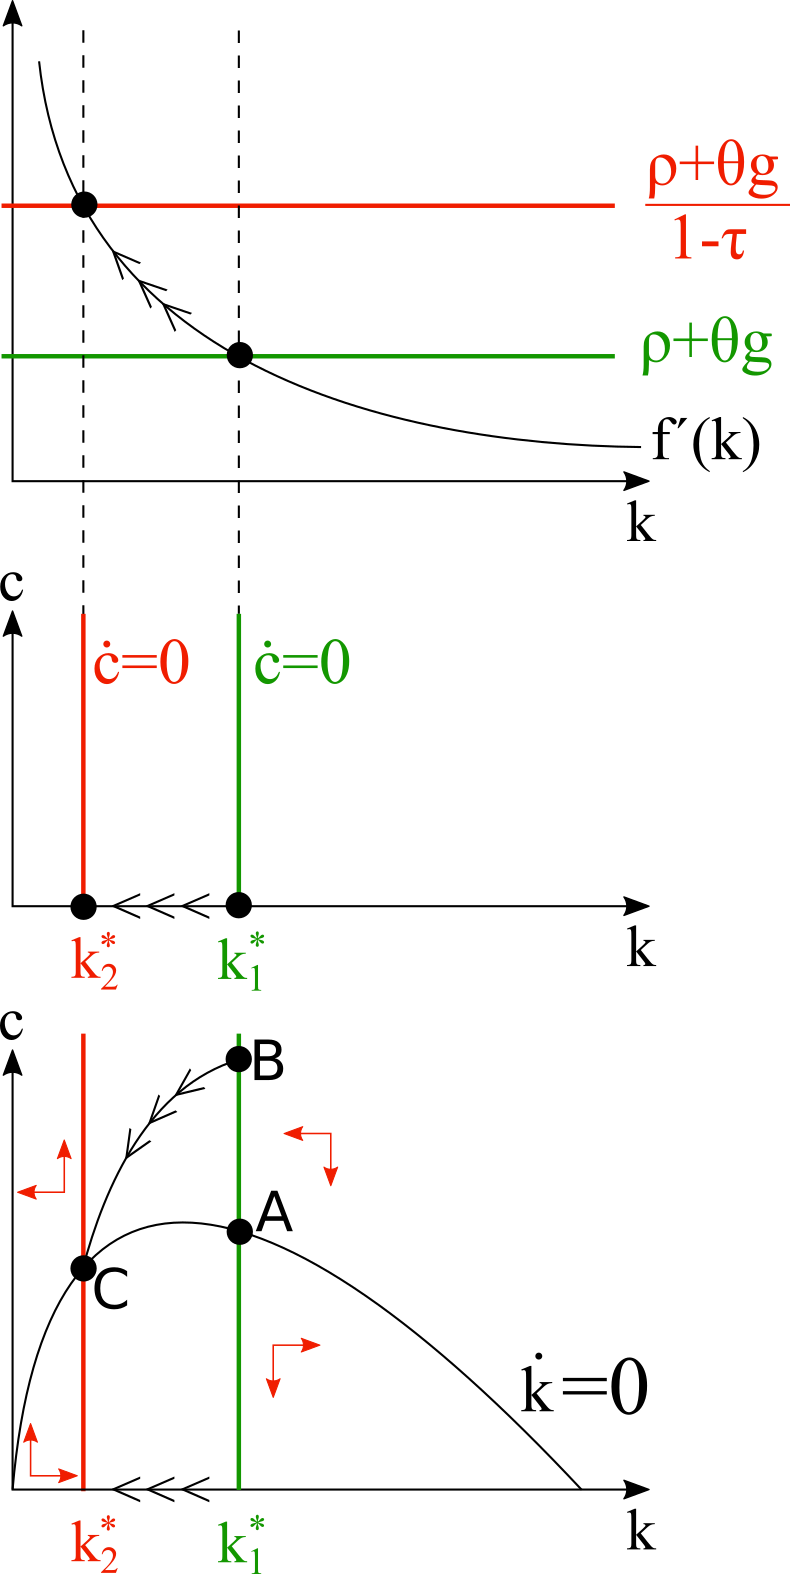
\includegraphics[width=0.48\textwidth]{2.b}
  \end{center}
  \caption{Dynamics of implementing an investment tax.}
\end{wrapfigure}


\vspace{3em}

We can see in the top panel to the left that the level of capital $k^*$ that satisfies the consumption Euler equation decreases from $\kone$ to $\ktwo$ when the new tax is introduced. This implies the change in the steady state level of consumption ($c$ where $\ccdot=0$) as we see in the middle panel. Before the tax is introduced, we assume that the economy was at point A in the bottom panel. Immediately after the unanticipated tax is introduced, the amount of capital has not had time to change, so it is still at $\kone$. The new steady state point with the tax is point C, where the new $\ccdot=0$ locus intersects the $\kdot=0$ locus. But in order to be on the saddle path to their new steady state C, consumers must increase their consumption from point A up to point B immediately after the tax is introduced (an instantaneous jump in this model).

Thus, consumers first jump to point B, then follow their saddle path to point C in order to follow their Euler equation. Where the concavity of the saddle path is determined by the utility parameter $\theta$.

}

%%%%%%%%%%%%%%%%%
%     Part c    %
%%%%%%%%%%%%%%%%%
\newpage\problem{}{
    \begin{enumerate}[label=(\alph*)]
    \setcounter{enumi}{2}
    \item How do the values of $c$ and $k$ on the new balanced growth path compare with their values on the old balanced growth path?
    \end{enumerate} 
}

\begin{itemize}
    \item $k$ at the time of the change remains $\kone$, where it was on the old balanced growth path.
    \item $k$ after the change decreases monotonically to $\ktwo$, which is lower than on the old balanced growth path.
    \item $c$ at the time of the change jumps up discontinuously from the old balanced-growth-path value to the new saddle path (higher than where it was on the old balanced growth path).
    \item $c$ after the change decreases monotonically to the new balanced growth path, and it will end at the new balanced growth path, which could be above or below the consumption on the old balanced growth path depending on the parameters and shape of $f(k)$.
\end{itemize}

%%%%%%%%%%%%%%%%%
%     Part d    %
%%%%%%%%%%%%%%%%%
\newpage\problem{}{
    \begin{enumerate}[label=(\alph*)]
    \setcounter{enumi}{3}
    \item (This is based on Barro, Mankiw, and Sala-i-Martin, 1995.) Suppose there are many economies like this one. Workers’ preferences are the same in each country, but the tax rates on investment income may vary across countries. Assume that each country is on its balanced growth path.
    
    \begin{enumerate}[label=(i)]
        \item Show that the saving rate on the balanced growth path, $(y^* - c^*)/y^*$, is decreasing in $\tau$.
    \end{enumerate}
    \end{enumerate} 
}

\begin{align*}
    \intertext{Denote optimal savings rate as $s^* = (y^* - c^*)/y^*$. First we can use the $\kdot=0$ condition of the balanced growth path, which implies:}
    \c &= \y - (n+g)\k
    \intertext{Then the savings rate on the balanced growth path is}
    \s &= \frac{\y-\c}{\y} \\[1em]
        &= \frac{(n+g)\k}{\y} \\[1em]
        &= \frac{(n+g)\k}{\f}
    \intertext{Differentiating with respect to the tax rate, we have}
    \frac{d\s}{d\t} 
        &= (n+g)\l[\frac{1}{\f}\frac{d\k}{d\t} - \frac{\k}{\f^2}\frac{df(\k)}{d\t} \r] \\[1em]
        &= (n+g)\l[\frac{1}{\f}\frac{d\k}{d\t} - \frac{\k}{\f^2}f'(\k)\frac{d\k}{d\t} \r] \\[1em]
        &= \frac{n+g}{\f^2}\l[\f - \k f'(\k)\r]\frac{d\k}{d\t} \\[1em]
    \intertext{Since $\dfrac{n+g}{\f^2}>0$, we just need to determine the sign of the last two terms. Starting with the term in the brackets: from our assumptions about the production function, we can determine that}
    f'>0, f''<0 &\implies f(k) > k f'(k) \\
        &\implies f(k) - k f'(k) > 0 \quad \forall k>0
    \intertext{We can think about this graphically: since the slope of $f$ is positive and always decreasing, the tangent to $f$ at any point is going to intersect the vertical axis above the origin (i.e., $>0$). $f(k) - k f'(k)$ is precisely the height above the origin where this tangent intersects the vertical axis. The figure below demonstrates this for a particular point $k$, but it holds generally anywhere in the domain of $f$.}
\end{align*}
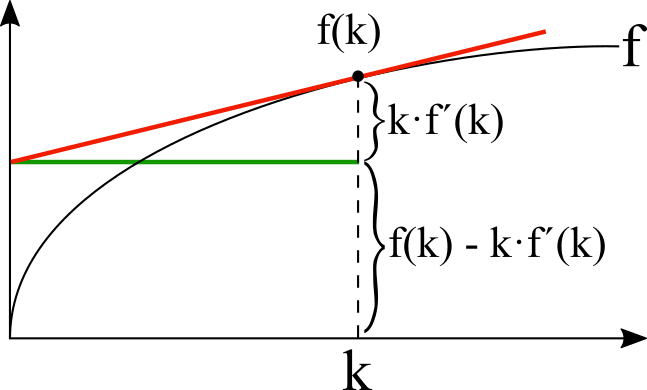
\includegraphics[width=0.5\textwidth]{1.f}
\begin{align*}
    \intertext{For the last term, we can use the $\ccdot=0$ condition to find the balanced-growth-path level of capital and differentiate. The $\ccdot=0$ condition implies}
    f'(\k) &= \frac{\rho + \theta g}{1-\t} \\[1em]
    \implies \k &= f'{}^{-1}\l( \frac{\rho + \theta g}{1-\t}\r) \\[1em]
    \implies \frac{d\k}{d\t} &= \frac{d}{d\t} f'{}^{-1}\l( \frac{\rho + \theta g}{1-\t}\r) \\[1em]
        &= f'{}^{-1}{}'\l( \frac{\rho + \theta g}{1-\t}\r)
            \frac{\rho + \theta g}{(1-\t)^2} \\[1em]
    \intertext{where $'$ indicates the derivative of the univariate function and $f'{}^{-1}{}'\equiv (f'(\cdot)^{-1})'$.}
    \intertext{By assumption, $f'>0, f''<0$, and}
    f'>0, f''<0 &\implies f'{}^{-1}>0, f'{}^{-1}{}' <0
    \intertext{We can again think about this graphically. $f'>0$ so it is in the first quadrant. $f''<0$ so it is decreasing in $k$. Taking the inverse of a function in the first quadrant is the same as reflecting it across the 45$^\deg$ line, so a positive, decreasing function will have an inverse that is also positive and decreasing. Meaning, $f'{}^{-1}>0, f'{}^{-1}{}' <0$. This implies}
    \frac{d\k}{d\t} &= f'{}^{-1}{}'\l( \frac{\rho + \theta g}{1-\t}\r)
            \frac{\rho + \theta g}{(1-\t)^2} \\[1em]
            &<0
    \intertext{Which means that}
    \frac{d\s}{d\t} &= \underbrace{ \frac{n+g}{\f^2} }_{>0}
            \underbrace{ \l[\f - \k f'(\k)\r] }_{>0}
            \underbrace{ \frac{d\k}{d\t} }_{<0} \\[1em]
        &<0
    \intertext{So the endogenous savings rate on the balanced growth path decrease as the investment income tax increases.}
\end{align*}


%%%%%%%%%%%%
% Part ii %
%%%%%%%%%%%
\newpage\problem{}{
    \begin{enumerate}[label=(ii)]
    \item Do citizens in low-$\tau$, high-$k^*$, high-saving countries have any incentive to invest in low-saving countries? Why or why not?
    \end{enumerate} 
}

The $\ccdot=0$ condition implies that $r(t) = \rho + \theta g$, hence the steady-state real interest rate is constant \textit{and independent of the tax rate} $\t$ (Barro et al. 1995). Since all countries share the fundamental parameters $\rho, \theta$, and $g$, the steady-state real interest rate is the same for all countries. Because the real interest is the same, there is no incentive for low-$\tau$, high-$k^*$ countries to invest in low-$k^*$ (low savings) countries. This is a result of the simplicity of the model and Barro goes on to discuss how including capital frictions play a role in predicting the rates of convergence of poor and rich countries -- namely that including those frictions only changes the speed of convergence a small amount.
 

%%%%%%%%%%%%%%%%%
%     Part e    %
%%%%%%%%%%%%%%%%%
\newpage\problem{}{
    \begin{enumerate}[label=(\alph*)]
    \setcounter{enumi}{4}
    \item Does your answer to part (c) imply that a policy of \textit{subsidizing} investment (that is, making $\tau<0$), and raising the revenue for this subsidy through lump-sum taxes, increases welfare? Why or why not?
    \end{enumerate} 
}

In all cases, subsidizing investment will move the $\ccdot=0$ curve to a higher $k^*$. This is because $(1-\t)>1$ and $\dfrac{\rho+\theta g}{1-\t}<\rho+\theta g$, therefore the $\dfrac{\rho+\theta g}{1-\t}$ will intersect $f'(k)$ at a higher $k$ (and this intersection is the solution to the $\ccdot=0$ condition). But whether this higher $k^*$ induces higher welfare depends on where our starting balanced growth path $k-c$ point is (where $\ccdot=0$ and $\kdot=0$). 

\begin{itemize}
    \item If the shift to a higher $k^*$ along the $\kdot=0$ curve results in a higher $c^*$, then steady-state consumption has increased and welfare has improved.
    \item If the shift to a higher $k^*$ along the $\kdot=0$ curve results in a lower $c^*$, then steady-state consumption has decreased and welfare has decreased.
\end{itemize}

If we are not already at the golden rule level of capital, then there exists some tax or subsidy that would induce a welfare increase and shift to the golden rule level of captial.




%%%%%%%%%%%%%%%%%
%     Part f    %
%%%%%%%%%%%%%%%%%
\newpage\problem{}{
    \begin{enumerate}[label=(\alph*)]
    \setcounter{enumi}{5}
    \item How, if at all, do the answers to parts (a) and (b) change if the government does not rebate the revenue from the tax but instead uses it to make government purchases?
    \end{enumerate} 
}

The government spending does not change the $\ccdot$ equation from parts (a) and (b), thus the $k^*$ remains the same. However, the new $\kdot=0$ equation becomes $c=f(k)-(n+g)k-G$, where $G$ is the government spending of the tax revenue. This just means that the $\kdot=0$ curve is translated downward by $G$ units of consumption. The economy jumps to the new balanced growth path at the same $k^*$ and lower $c^*$. 

From the figure in part (b), the point C in the bottom panel would simply be shifted downward. So depending on how large $G$ is (or $\t$), point B would either be below or above point A. So if $G$ was large enough, point B could be below point A, and consumption might jump down instead of up in order to get on the new saddle path to the balanced growth path (the new point C).





\end{document}

